\chapter{Kennismaking met Spring Boot}
    
\fcolorbox{black}[HTML]{E9F0E9}{\parbox{\textwidth}{%
\noindent \textbf{Learning goals}\\
De junior-collega
\begin{enumerate}[nolistsep]
\item kan beschrijven wat het Spring framework is
\item kan beschrijven wat Spring Boot is
\item kan de kenmerken van een enterprise toepassing benoemen
\item kan uitleggen wat inversion of control (IoC) is
\item kan uitleggen wat dependency injection is
\item kan beschrijven wat een Spring Bean is
\item kan beschrijven wat de Application Context is
\item kan een nieuwe Spring Boot applicatie aanmaken en opstarten
\item kan Spring Beans aanmaken en gebruiken
\end{enumerate}}}


\section{Enterprise toepassingen met Java}

Spring Boot is een framework om enterprise toepassingen te bouwen met Java.
Enterprise toepassingen zijn toepassingen die bedrijven bouwen of laten bouwen voor hun klanten en medewerkers.  Enterprise toepassingen worden ontwikkeld om bedrijfsprocessen te ondersteunen. 

Enterprise toepassingen hebben specifieke kenmerken omwille van de complexe aard en specifieke eisen van grootschalige bedrijfssystemen.  Enkele belangrijke kenmerken van enterprise toepassingen vanuit het oogpunt van een ontwikkelaar zijn:

\begin{itemize}
\item{\textbf{Schaalbaarheid (scalability):}} Enterprise applicaties moeten een groot aantal gebruikers en gegevens aankunnen.  Ontwikkelaars moeten de architectuur van de toepassing zodanig ontwerpen dat schalen mogelijk is om een groeiend aantal gebruikers en datavolumes aan te kunnen.

\item{\textbf{Betrouwbaarheid en hoge beschikbaarheid:}} Van enterprise applicaties wordt verwacht dat ze 24/7 beschikbaar zijn en snelle responstijden hebben.  Ontwikkelaars moeten oplossingen voorzien om problemen en downtime te voorkomen.  Ze moeten de betrouwbare werking van de applicatie kunnen garanderen.

\item{\textbf{Beveiliging:}} Enterprise applicaties verwerken gevoelige bedrijfsgegevens, waaronder financiële informatie, klantgegevens,...   Ontwikkelaars moeten robuuste beveiligingsmaatregelen implementeren,  zoals authenticatie,  autorisatie,  versleuteling van gegevens, audittrails, .\vdots om de gegevens te beschermen tegen ongeautoriseerde toegang.

\item{\textbf{Integratie:}} Enterprise applicaties moeten vaak worden geïntegreerd met verschillende bestaande systemen zoals databanken en externe services.  Voorbeelden van externe services zijn bijvoorbeeld betaalsystemen en boekhoudpakketten. Ontwikkelaars moeten zorgen voor een veilige en betrouwbare gegevensuitwisseling tussen verschillende enterprise applicaties. 

\item{\textbf{Aanpasbaarheid en flexibiliteit:}} Enterprise applicaties worden gebruikt door gebruikers uit diverse afdelingen en teams binnen een organisatie, elk met hun eigen unieke workflows en eisen. Ontwikkelaars moeten applicaties bouwen die kunnen worden aangepast en geconfigureerd om aan deze specifieke behoeften te voldoen. 
Enterprise applicaties ondergaan vaak veranderingen en updates op basis van veranderende zakelijke behoeften. Daarnaast veranderen de workflows en eisen van de gebruikers ook. 
Ontwikkelaars moeten verandering effectief beheren door versiebeheer, wijzigingstracering en terugrolmechanismen te implementeren.
Afhankelijk van de sector moeten enterprise applicaties voldoen aan specifieke wettelijke normen die doorheen de tijd kunnen veranderen. 

\item{\textbf{Lange levenscyclus:}} Enterprise applicaties hebben meestal een langere levenscyclus dan andere soorten software.  Ontwikkelaars moeten zorgen voor voortdurend onderhoud,  updates en verbeteringen.

\item{\textbf{Samenwerking en documentatie:}} Aangezien meerdere ontwikkelaars en teams werken aan verschillende delen van een enterprise applicatie, zijn duidelijke codeerrichtlijnen,  versiebeheer en samenwerkingstools essentieel.

\item{\textbf{Testen en kwaliteitsborging:}} Grondig testen is essentieel voor enterprise applicaties om bugs, prestatieproblemen en kwetsbaarheden in de beveiliging te identificeren en aan te pakken. Ontwikkelaars moeten unit test,  integratietesten en gebruikersacceptatietesten implementeren. Al deze testen worden geautomatiseerd en bij iedere aanpassing aan de code uitgevoerd.

\item{\textbf{Gebruikerservaring (UX):}} Hoewel functionaliteit cruciaal is, is een positieve gebruikerservaring ook belangrijk. Ontwikkelaars moeten streven naar intuïtieve interfaces en workflows zodat de gebruikers productief zijn.
\end{itemize}

Over het algemeen vereist de ontwikkeling van enterprise applicaties een uitgebreid begrip van bedrijfsprocessen, technische expertise en het vermogen om functionaliteit, performantie, beveiliging en gebruikerservaring in evenwicht te brengen om te voldoen aan de unieke behoeften van grote organisaties.

In 1999 besliste Sun Microsystems om de programmeertaal Java uit te bereiden om het ontwikkelen van enterprise applicaties te vergemakkelijken.  Met de lancering van J2EE (Java 2 Enterprise Edition) en de applicatie servers om de J2EE-toepassingen op te deployen onstond een schaalbaar en betrouwbaar platform. 
J2EE,  dat werd hernoemd naar Java EE (Java Platform,  Enterprise Edition), verwijst naar een verzameling specificaties voor het ontwikkelen van enterprise applicaties.  Het bestaat uit een reeks standaarden en API's die ontwikkelaars gebruiken om de enterprise-software te implementeren. 

Wanneer we spreken over "J2EE-specificaties" of "Java EE-specificaties", dan verwijst dit naar de reeks specificaties die samen Java EE vormen.  Deze specificaties zijn de  beschrijvingen van hoe bepaalde componenten en functionaliteiten in een enterprise Java-applicatie moeten worden geïmplementeerd.  Sun Microsystems en later Oracle, dat in de 2010 Sun Microsystems overnam, zorgen steeds voor een bruikbare implementatie van de specificaties. 

Laten we het versturen van mails als voorbeeld nemen. In bijna iedere enterprise applicatie moet het mogelijk zijn om op een eenvoudige manier mails te versturen.
Daarom werden de JavaMail API Design Specifications uitgeschreven. Dit kan je zien als een uitgebreide analyse van de vereisten.  De reference implementation is voorzien door Oracle zelf. Naast de reference implementation zijn er nog andere spelers op de markt die hun implementatie, vaak met bijkomende functionaliteiten, aanbeiden. Voor de JavaMailAPI kan je bijvoorbeeld kiezen uit Apache Geronimo JavaMail, WildFly (JBoss) JavaMail, Google App Engine JavaMail, \vdots

Het Spring framework ontstond in 2003 als reactie op de complexiteit van de JEE-specificaties.  Sommigen zien Spring als een concurrent van Java EE en zijn moderne opvolger Jakarta EE.  Maar als je Spring leert kennen zal je merken dat Spring zorgvuldig individuele specificaties uit Jakarta EE integreert.  Waar de ontwikkeling van Enterprise JavaBeans (EJB's) in een JEE toepassing eerder omslachtig was,  bood Spring een eenvoudigere benadering met Spring Beans. Toch bleeft het Spring framework complex omwille van de configuratie. Deze configuratie gebeurde initieel door (veel) XML bestanden.  Vanaf Spring Framework 6.0 is Java 17+ vereist.

Spring Boot is een open-source Java framework dat gebouwd is boven op het Spring Framework. 
En het biedt uiteraard alles om enterprise applicaties te ontwikkelen in Java.
Het biedt een eenvoudigere en snellere manier een toepassing te cre\"eren, te configureren en uit te voeren.

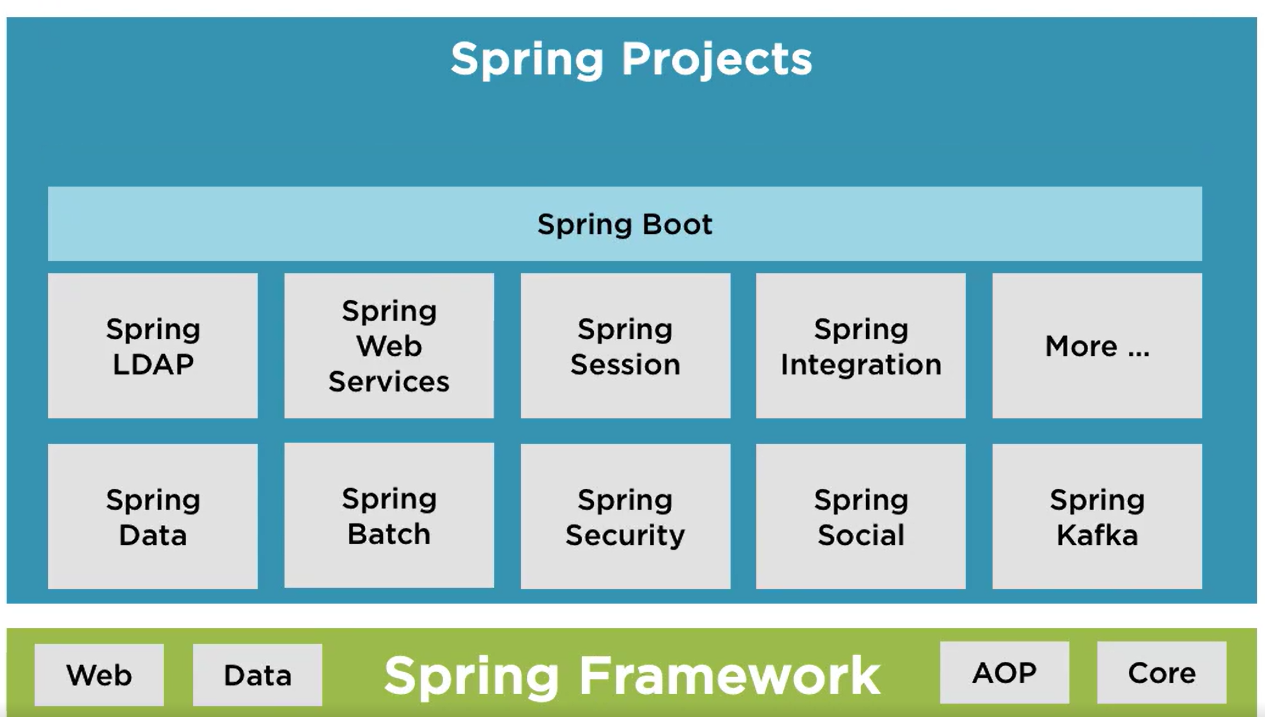
\includegraphics[width=\textwidth]{./images/chapter1/spring_framework.png} 
    
Spring Boot  biedt verschillende voordelen voor ontwikkelaars.

\begin{itemize}
\item Gemakkelijker en sneller creëren en implementeren van enterprise applicaties.
\item Minder of bijna geen configuratie.
\item Eenvoudiger te leren framework.
\item Verhoogt de productiviteit.
\end{itemize}

\section{Bootstrapping van een eenvoudige Spring Boot applicatie}

\subsection{Gebruik van Spring Initializr}
Spring Initializr is een webtoepassing waarmee je een Spring Boot-project kunt genereren. De URL voor deze webtoepassing is \url{https://start.spring.io/}. Je kunt de benodigde configuratie selecteren zoals de buildtool,  programmeertaal,  versie van het Spring Boot-framework en eventuele afhankelijkheden voor je project.  IntelliJ IDEA Ultimate biedt de Spring Initializr-projectwizard die integreert met de Spring Initializr API om je project rechtstreeks in de IDE te genereren en te importeren.

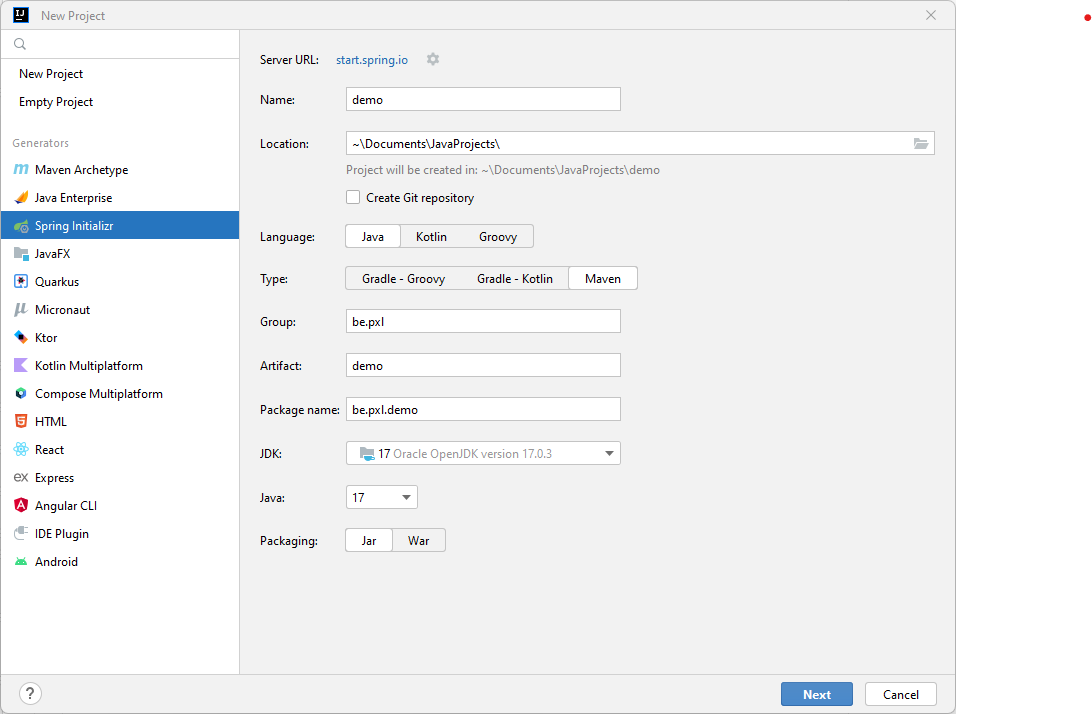
\includegraphics[width=\textwidth]{./images/chapter1/spring_initializer_intellij.png}

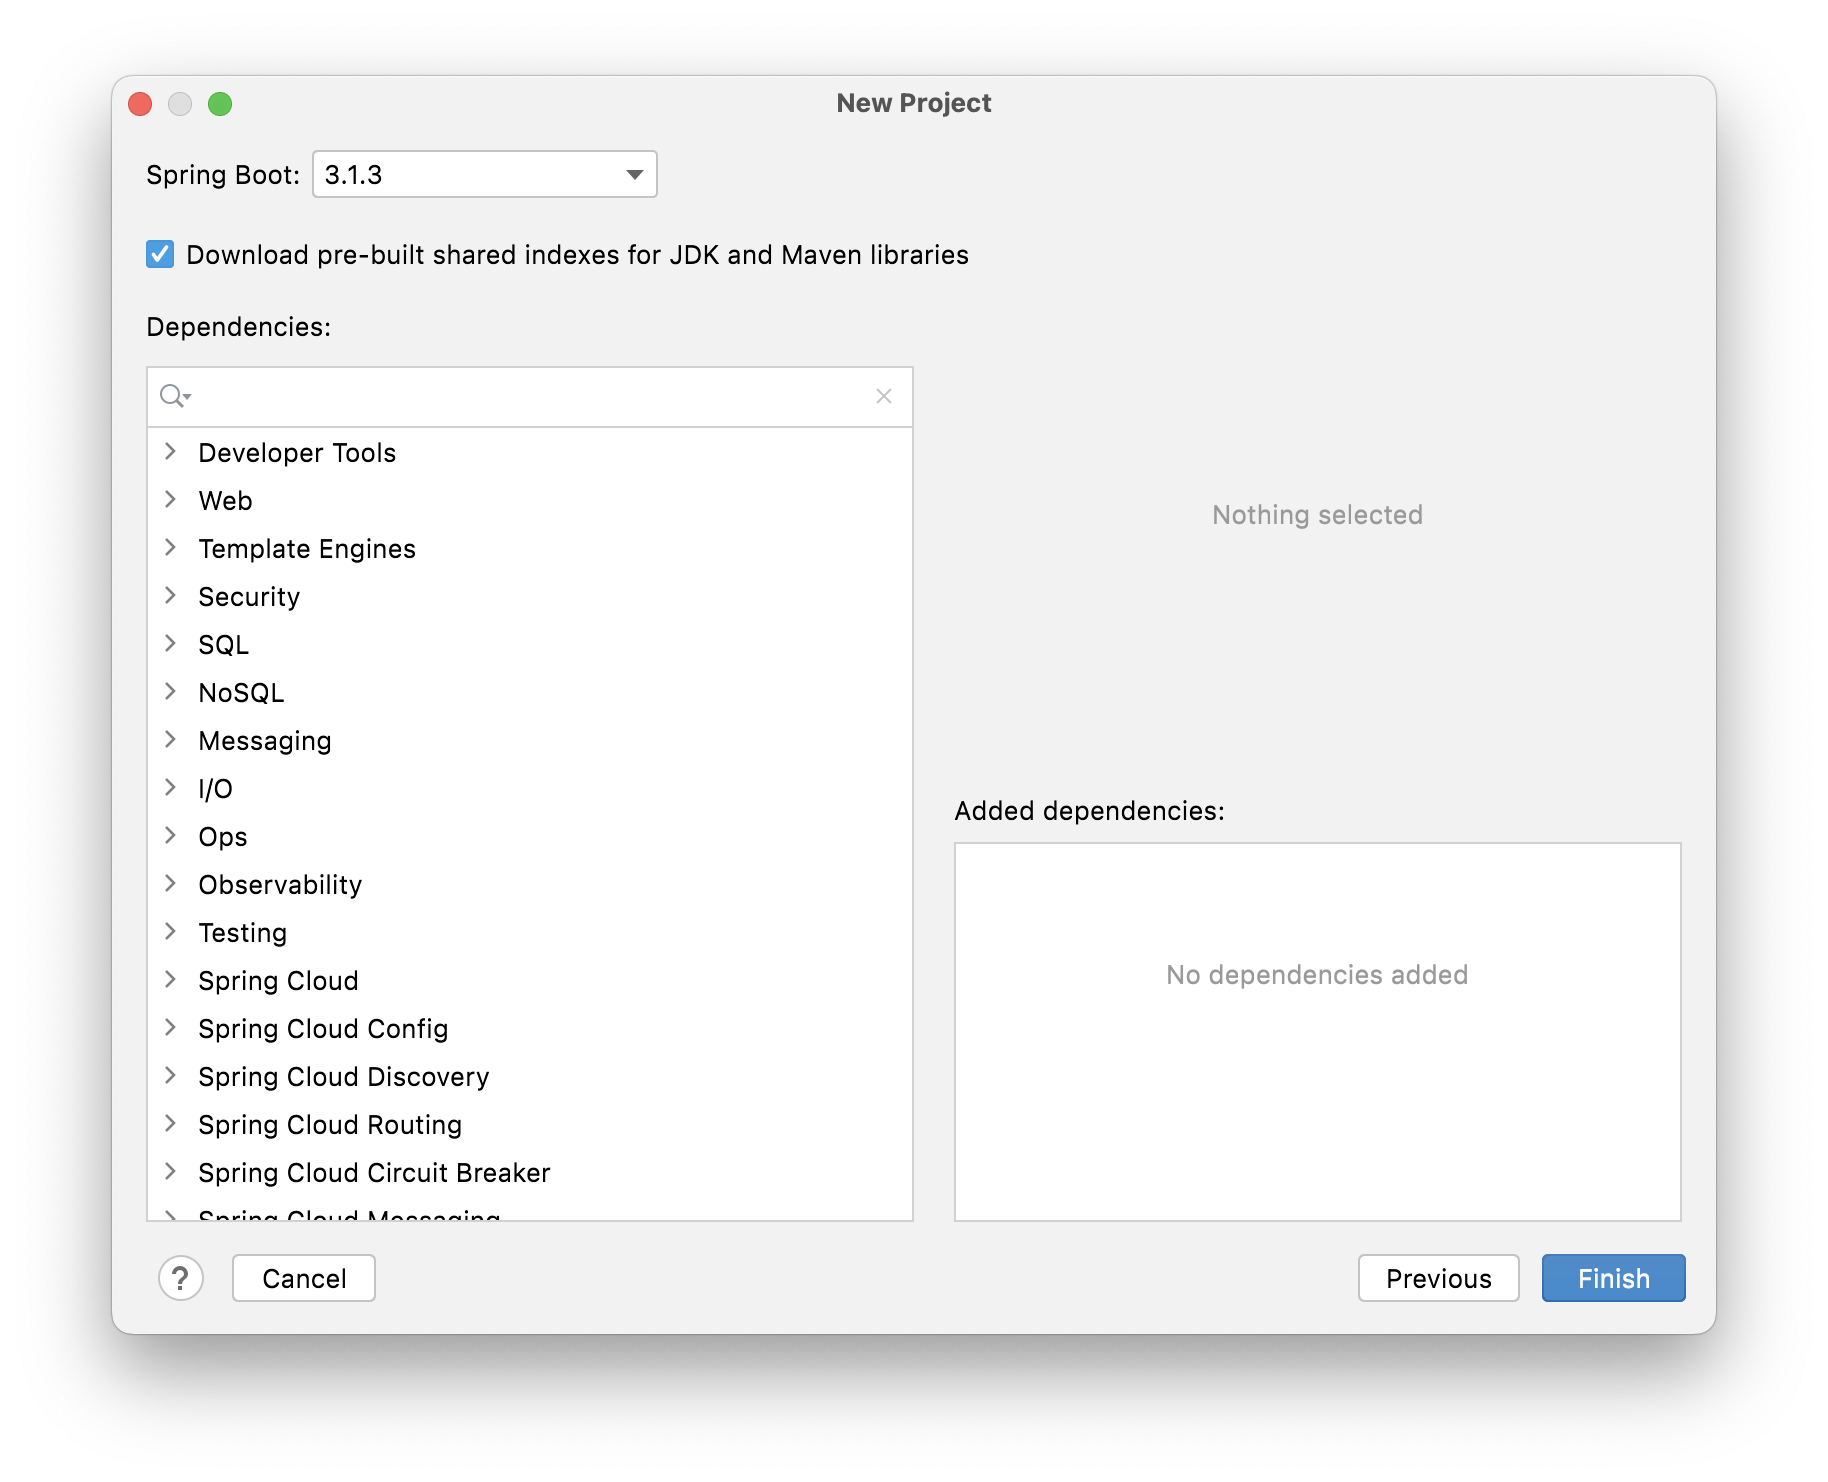
\includegraphics[width=\textwidth]{./images/chapter1/new_project.png}

Wanneer je Maven als buildtool kiest krijgt je nieuw project de typische folder-structuur van Maven. 

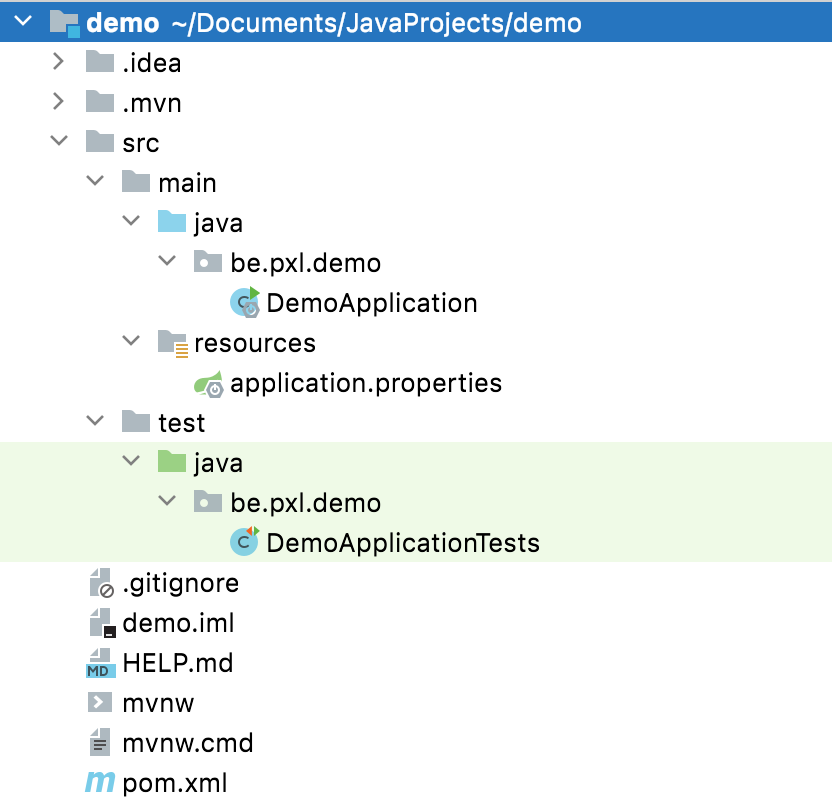
\includegraphics[width=\textwidth]{./images/chapter1/new_project_files.png}

De eigenlijke broncode komt in de src folder. De testen, die we later leren schrijven, komen in de test folder terecht.

\begin{oefening}
Maak het demo-project aan zoals in de screenshots. Je kan de wizard van IntelliJ IDEA Ultimate of de webtoepassing \url{https://start.spring.io/} gebruiken.
\end{oefening}

\section{Het demo-project uitvoeren}

Het startpunt van een Spring Boot toepassing is de klasse met de main-methode.
Deze klasse is geannoteerd met \textbf{@SpringBootApplication}. Je vind deze klasse terug in de folder /src/main/java in het package be.pxl.demo.  Spring Boot biedt heel veel functionalteit aan in de vorm van annotaties om het werk van de ontwikkelaars te vereenvoudigen.   

\begin{lstlisting}[frame=single, language=java]
package be.pxl.demo;

import org.springframework.boot.SpringApplication;
import org.springframework.boot.autoconfigure.SpringBootApplication;

@SpringBootApplication
public class DemoApplication {

	public static void main(String[] args) {
		SpringApplication.run(DemoApplication.class, args);
	}
}
\end{lstlisting}

Start nu de Spring Boot applicatie op.

\begin{small}
\begin{verbatim}
  .   ____          _            __ _ _
 /\\ / ___'_ __ _ _(_)_ __  __ _ \ \ \ \
( ( )\___ | '_ | '_| | '_ \/ _` | \ \ \ \
 \\/  ___)| |_)| | | | | || (_| |  ) ) ) )
  '  |____| .__|_| |_|_| |_\__, | / / / /
 =========|_|==============|___/=/_/_/_/
 :: Spring Boot ::                (v3.1.3)

2023-09-13T09:49:42.340+02:00  INFO 81620 --- [main] be.pxl.demo.DemoApplication: Starting DemoApplication using Java 17.0.1 with PID 81620 (/Users/nelec/Documents/JavaProjects/demo/target/classes started by nelec in /Users/nelec/Documents/JavaProjects/demo)
2023-09-13T09:49:42.343+02:00  INFO 81620 --- main] be.pxl.demo.DemoApplication: No active profile set, falling back to 1 default profile: "default"
2023-09-13T09:49:42.858+02:00  INFO 81620 --- [main] be.pxl.demo.DemoApplication: Started DemoApplication in 0.734 seconds (process running for 1.256)

Process finished with exit code 0
\end{verbatim}
\end{small}

Java annotations are a mechanism for adding metadata information to our source code. An annotation processor processes these annotations at compile time or runtime to provide functionality such as code generation, error checking, etc.

\section{De Maven POM file}

POM staat voor \'Project Object Model\'. Omdat we voor Maven hebben gekozen als buildtool van onze Spring Boot-toepassing staan hier de project-co\"ordinaten in. Alle dependencies die door ons project worden gebruikt staan hier opgelijst en worden door maven gedownload.

\begin{lstlisting}[frame=single]
?xml version="1.0" encoding="UTF-8"?>
<project xmlns="http://maven.apache.org/POM/4.0.0" xmlns:xsi="http://www.w3.org/2001/XMLSchema-instance"
         xsi:schemaLocation="http://maven.apache.org/POM/4.0.0 https://maven.apache.org/xsd/maven-4.0.0.xsd">
	<modelVersion>4.0.0</modelVersion>
	<parent>
		<groupId>org.springframework.boot</groupId>
		<artifactId>spring-boot-starter-parent</artifactId>
		<version>3.1.3</version>
		<relativePath/> <!-- lookup parent from repository -->
	</parent>
	<groupId>be.pxl</groupId>
	<artifactId>demo</artifactId>
	<version>0.0.1-SNAPSHOT</version>
	<name>demo</name>
	<description>demo</description>
	<properties>
		<java.version>17</java.version>
	</properties>
	<dependencies>
		<dependency>
			<groupId>org.springframework.boot</groupId>
			<artifactId>spring-boot-starter</artifactId>
		</dependency>

		<dependency>
			<groupId>org.springframework.boot</groupId>
			<artifactId>spring-boot-starter-test</artifactId>
			<scope>test</scope>
		</dependency>
	</dependencies>

	<build>
		<plugins>
			<plugin>
				<groupId>org.springframework.boot</groupId>
				<artifactId>spring-boot-maven-plugin</artifactId>
			</plugin>
		</plugins>
	</build>

</project>

\end{lstlisting}
De spring-boot-starter-parent is het basisproject dat alle standaardconfiguratie biedt voor op Spring gebaseerde toepassingen. Hier kies je de versie van Spring Boot.

Voor grote projecten is het beheren van afhankelijkheden (dependencies) niet altijd eenvoudig. Spring Boot lost dit probleem op door bepaalde afhankelijkheden samen te bundelen. Deze groepen van afhankelijkheden worden starters genoemd. Alle Spring Boot starters volgen dezelfde richtlijnen voor hun naamgeving.  Ze beginnen allemaal met spring-boot-starter-*, waarbij * aangeeft welke functionaliteiten de starter aanbiedt.

spring-boot-starter-test (met scope test) is de starter voor het testen van Spring Boot-toepassingen met o.a. JUnit Jupiter, Hamcrest en Mockito.

\section{Inversion of Control (IoC) en dependency injection}

\subsection{Spring Beans}

Spring Beans zijn componenten die volledig worden beheerd door het Spring Boot framework. Je hoeft zelf geen instanties van deze klassen te maken, Spring Boot genereert de objecten automatisch.  Daarnaast beheert Spring Boot ook de objecten. Wanneer een klasse gebruik wil maken van de functionaliteiten van een dergelijke Spring Bean, zal Spring Boot ervoor zorgen dat de instantie van de Spring Bean beschikbaar is voor de betreffende klasse.

We gaan een eerste Spring Bean toevoegen in onze Spring Boot toepassing.
De CommandLineRunner interface voorziet de mogelijkheid om een stukje code uit te voeren zodra de Spring Boot applicatie ge\"initialiseerd is. 

\begin{lstlisting}
@Component
public class WelcomeMessage implements CommandLineRunner {
   
   @Override    
   public void run(String... args) throws Exception {
	   System.out.println("Welcome to Java Advanced");
   }
}
\end{lstlisting}


Zodra je de CommandLineRunner interface implementeert in een klasse kan je de run-methode overschrijven. In de run-methode plaats je de code die uitgevoerd moet worden
als de applicatie opstart.  Zodra de Spring Boot applicatie opstart worden een aantal initialisatie-fasen doorlopen.  Eerst wordt de \textbf{application context} aangemaakt en alle Spring beans worden geladen. Als de applicatie volledige is ge\"initialiseerd wordt de run-methode van de CommandLineRunner automatisch door het Spring boot framework aangeroepen.


\subsection{Application context}

Inversion of Control (IoC) is \'e\'en van de basisprincipes van het Spring framework.
Bij het software engineering principe Inversion of Control wordt het cre\"eren en beheren van objecten de verantwoordelijkheid van een apart onderdeel binnen het programma. Dit onderdeel noemen we een container. Binnen Spring Boot is deze container een object van de klasse ApplicationContext.  We spreken daarom kortweg over de application context om deze container binnen het programma te benoemen.

De application context is een slimme doos waarin alle beans, informatie en instellingen voor de Spring Boot-toepassing worden bewaard.  Je kunt de application context beschouwen als het brein van de Spring Boot-applicatie dat alles coördineert en beschikbaar maakt voor de verschillende onderdelen van het programma.

\begin{figure}[H]
  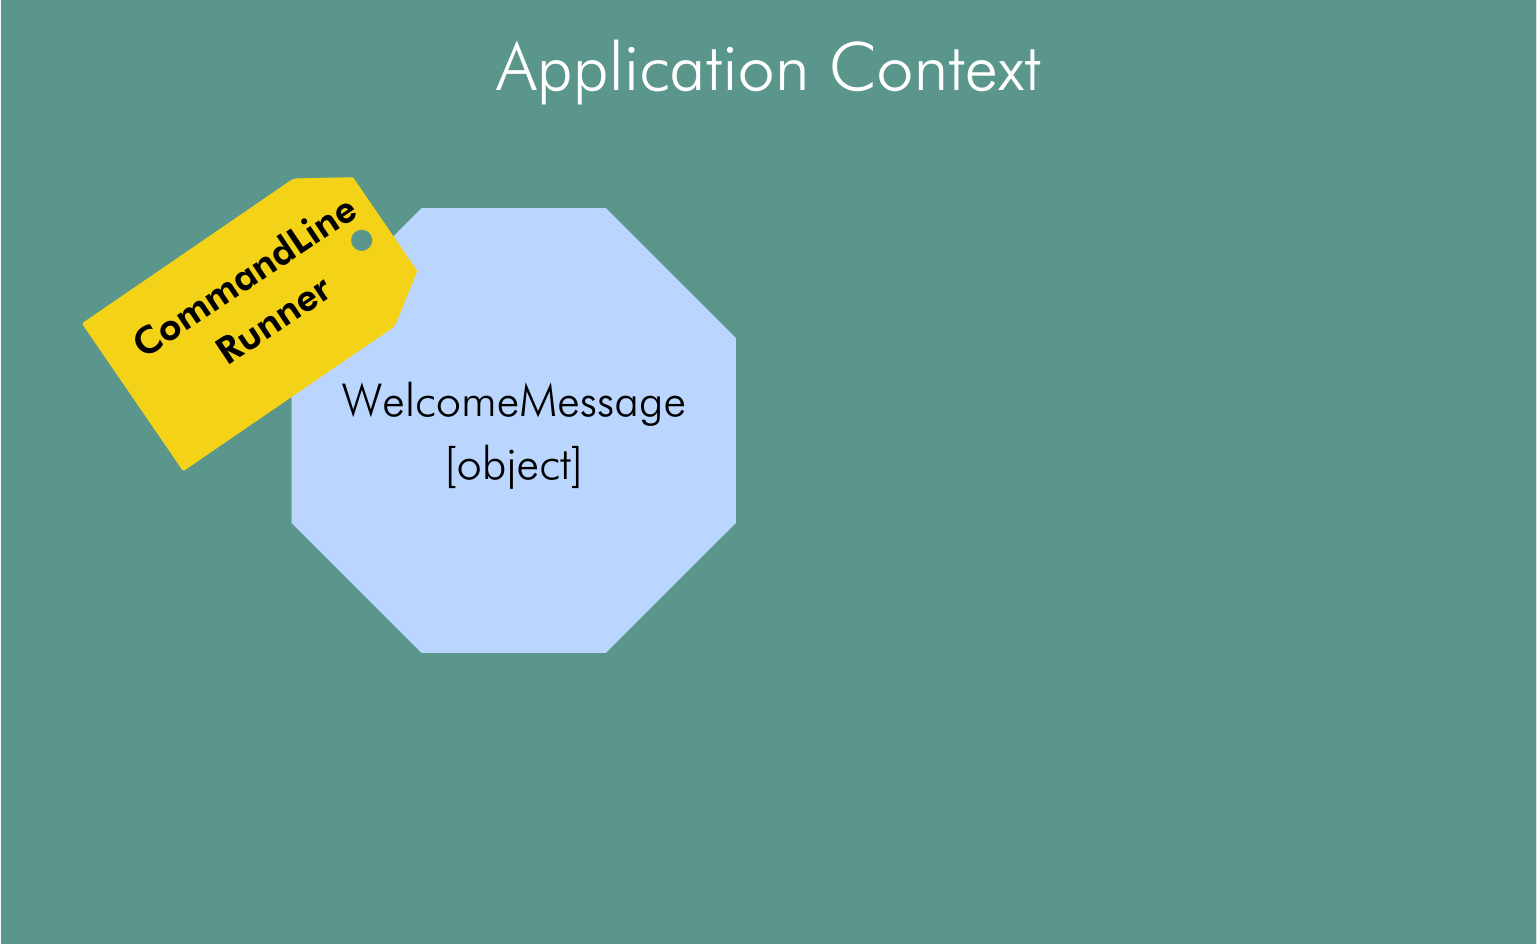
\includegraphics[width=\linewidth]{images/chapter1/application_context.png}
  \caption{De Application Context}
  \label{fig:application_context}
\end{figure}

Als de Spring Boot-applicatie opstart doorlopen we dus verschillende fasen in de initialisatie. Nadat de Application Context is aangemaakt, worden alle Spring beans geladen en daarna wordt de run-methode van de klassen die de CommandLineRunner interface implemeteren uitgevoerd.

De annotatie @SpringBootApplication zet eigenlijk 3 features van Spring Boot in werking. 
\begin{itemize}
\item Activeert het auto-configuratie mechanisme van Spring Boot (@EnableAutoConfiguration)
\item Activeert het scannen naar componenten met annotatie @Component (en ook @RestController,  @Service en @Repository) binnen het package  van de Spring Boot applicatie (@ComponentScan)
\item Laat toe dat binnen de klasse zelf extra beans worden gedefinieerd die door andere klassen gebruikt kunnen worden. (@Configuration)
\end{itemize}

We starten eerst met de klasse Pet (huisdier). We willen ons huisdier doorheen de ganse applicatie ter beschikking hebben.

\begin{lstlisting}
package be.pxl.demo;

public class Pet {
	private String name;
	private String breed;

	public Pet(String name, String breed) {
		this.name = name;
		this.breed = breed;
	}

	public String getBreed() {
		return breed;
	}

	public String getName() {
		return name;
	}

	@Override
	public String toString() {
		return "Pet{" +
				"name='" + name + '\'' +
				", breed='" + breed + '\'' +
				'}';
	}
}
\end{lstlisting}
 
Nu kunnen we dus in de main-klasse een Spring bean aanmaken voor ons favoriete huisdier.

\begin{lstlisting}
package be.pxl.demo;

import be.pxl.demo.domain.Pet;
import org.springframework.boot.SpringApplication;
import org.springframework.boot.autoconfigure.SpringBootApplication;
import org.springframework.context.ConfigurableApplicationContext;
import org.springframework.context.annotation.Bean;

@SpringBootApplication // can be replaced by @EnableAutoConfiguration @ComponentScan and @Configuration
public class DemoProjectApplication {

	public static void main(String[] args) {
		ConfigurableApplicationContext applicationContext = SpringApplication.run(DemoProjectApplication.class, args);
		System.out.println(applicationContext.getApplicationName());
		applicationContext.close();
	}

	@Bean
	public Pet myPet() {
		return new Pet("Scott", "Scotch Collie");
	}
}
\end{lstlisting}

Het Pet-object wordt bijgehouden in de application context.
Elke klasse die nu een Pet-object nodig heeft, kan dit object laten injecteren door de application context.
We spreken dan over \textbf{dependency injection}. We laten de application context als het ware objecten injecteren in andere objecten. Dat is dus de manier waarop Spring Boot zorgt dat inversion of control mogelijk is.

\begin{lstlisting}
package be.pxl.demo.beans;

import be.pxl.demo.domain.Pet;
import org.springframework.beans.factory.annotation.Autowired;
import org.springframework.boot.CommandLineRunner;
import org.springframework.stereotype.Component;

@Component
public class WelcomeMessage implements CommandLineRunner {
	private final Pet myPet;

	@Autowired // annotation not necessary
	public WelcomeMessage(Pet myPet) {
		this.myPet = myPet;
	}

	@Override
   public void run(String... args) throws Exception {
	   System.out.println("Welcome to Java Advanced");
		System.out.println(myPet);
   }
}
\end{lstlisting}

\begin{figure}[H]
  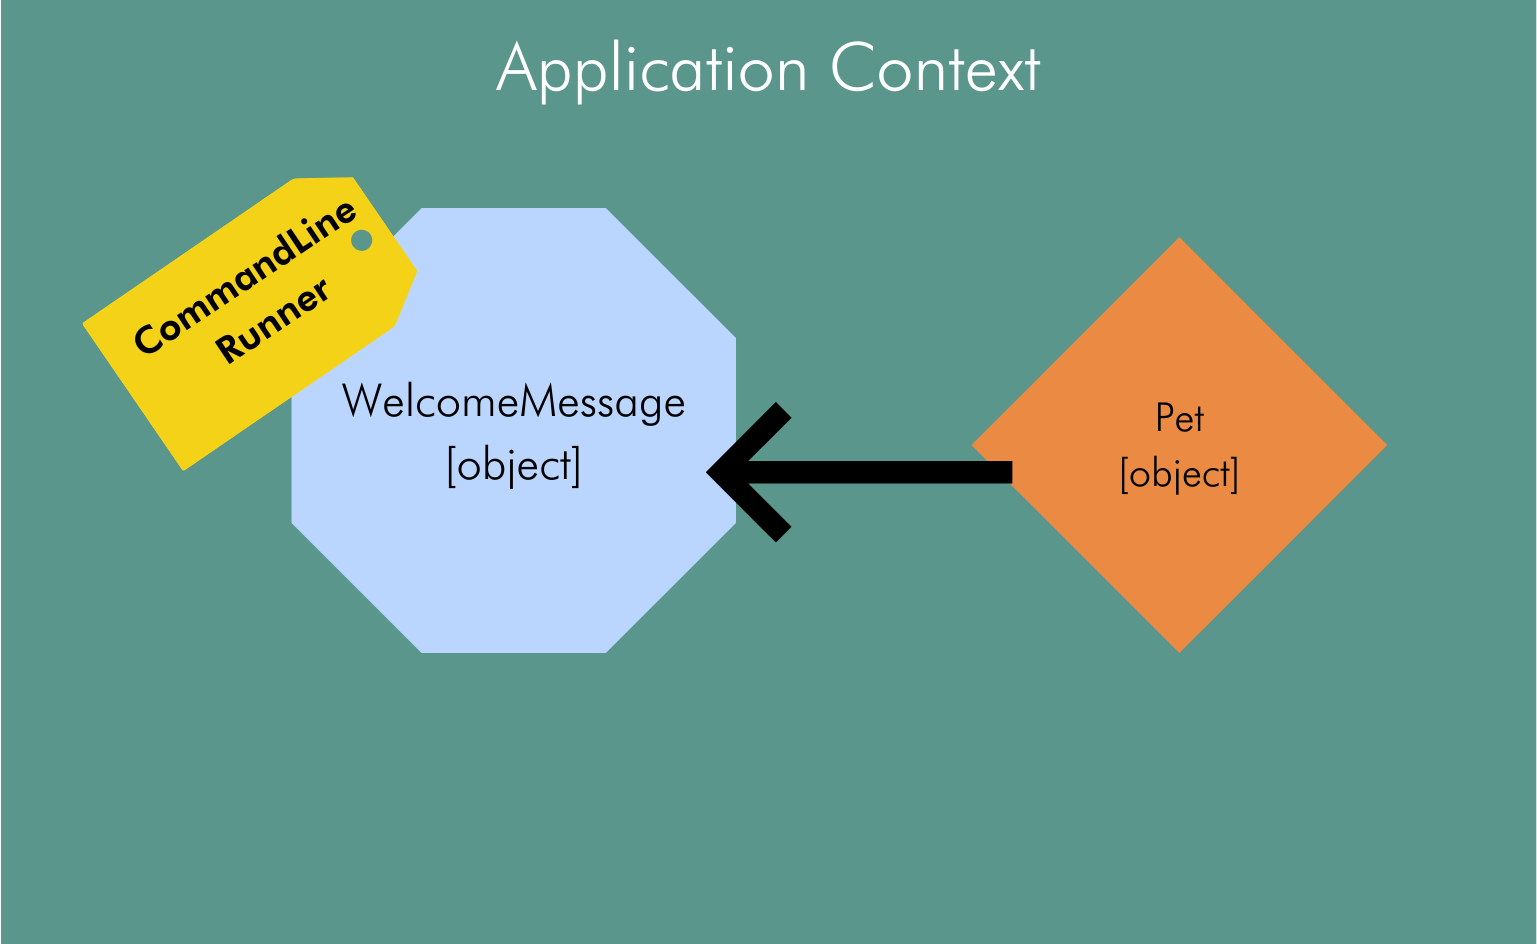
\includegraphics[width=\linewidth]{images/chapter1/application_context_with_pet.png}
  \caption{De Application Context}
  \label{fig:application_context}
\end{figure}

Wanneer je het programma uitvoert zal nu het volgende in de console verschijnen:
\begin{verbatim}
Welcome to Java Advanced
Pet{name='Scott', breed='Scotch Collie'}
\end{verbatim}

Om een idee te krijgen van de auto-configuratie die in de Spring Boot applicatie achter de schermen wordt uitgevoerd kan je het loglevel van de applicatie eens aanpassen.
Het loglevel van Spring Boot aanpassen doe je door een lijn toe te voegen in application.properties bestand dat je vindt in de folder /src/main/resources. 

\begin{lstlisting}
logging.level.org.springframework=debug
\end{lstlisting}

logging.level.org.springframework is \'e\'en van vele application properties.  Een overzicht van beschikbare application properties vind je terug op de documentatie website van Spring Boot \url{https://docs.spring.io/spring-boot/docs/current/reference/html/application-properties.html}.

In de logging vind je nu tussen de vele lijnen onderstaande regels:

\begin{small}
\begin{verbatim}
... Creating shared instance of singleton bean 'welcomeMessage'
... Creating shared instance of singleton bean 'myPet'
... Autowiring by type from bean name 'welcomeMessage' via constructor to bean named 'myPet'
\end{verbatim}
\end{small}

We geven nog een tweede voorbeeld van dependency injection.

\begin{lstlisting}
package be.pxl.demo.service;

import org.springframework.stereotype.Component;

@Component
public class WeatherService {
   public void printWeather() {
      System.out.println("The weather is sunny with a 20% chance of rain");
   }
}
\end{lstlisting}

We laten nu de instantie van de WeatherService injecteren in onze CommandLineRunnerWelcomeMessage.


\begin{figure}[H]
  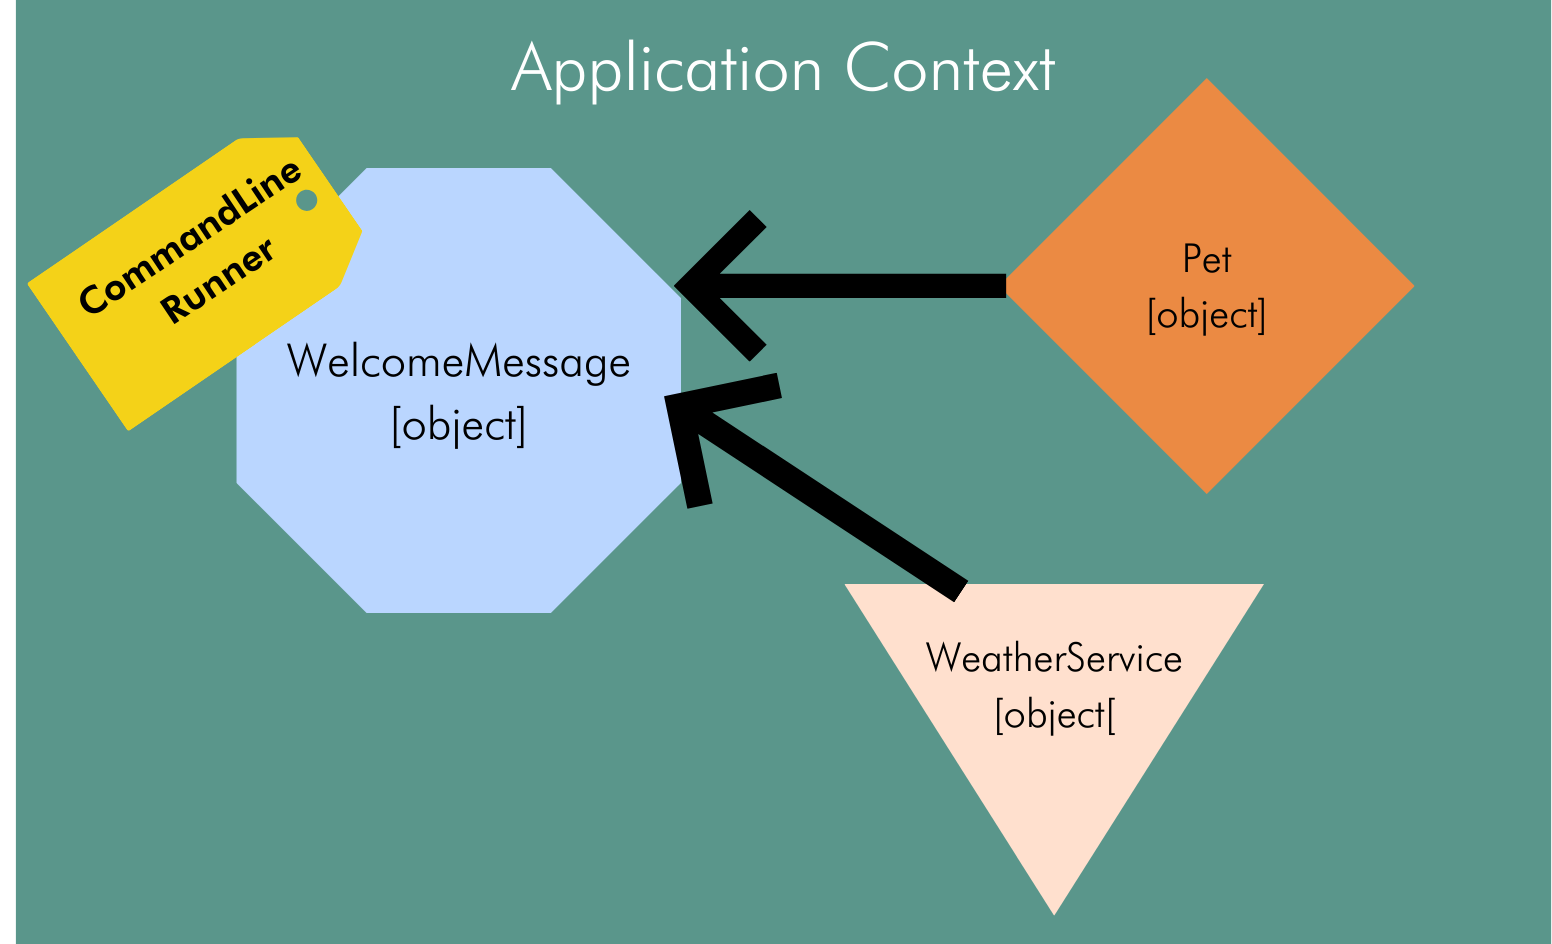
\includegraphics[width=\linewidth]{images/chapter1/ac_pet_service.png}
  \caption{De Application Context}
  \label{fig:application_context}
\end{figure}

\begin{lstlisting}
package be.pxl.demo.beans;

import be.pxl.demo.domain.Pet;
import be.pxl.demo.service.WeatherService;
import org.springframework.beans.factory.annotation.Autowired;
import org.springframework.boot.CommandLineRunner;
import org.springframework.stereotype.Component;

@Component
public class WelcomeMessage implements CommandLineRunner {

	private final Pet myPet;
	private final WeatherService weatherService;

	@Autowired // annotation not necessary
	public WelcomeMessage(Pet myPet, WeatherService weatherService) {
		this.myPet = myPet;
		this.weatherService = weatherService;
	}

	@Override
	public void run(String... args) throws Exception {
		System.out.println("Welcome to Java Advanced");
		System.out.println(myPet);
		weatherService.printWeather();
	}
}
\end{lstlisting}









